% Gabarit pandoc des corrigés publiés (brut et guidé). Contenu sans marque ni nom de site.
% Compilation : lualatex (latexmk -lualatex).
% Le Markdown reste la source unique : ne pas éditer ce fichier .tex à la main.
\documentclass[11pt,a4paper]{article}

% --- Moteur, polices (Latin Modern) et langue ---------------------------------
\usepackage{iftex}
\ifLuaTeX\else\errmessage{Ce document se compile avec lualatex}\fi
\usepackage{amsmath,amssymb,mathtools}
\usepackage{fontspec}
% mathrm=sym : \mathrm prend ses glyphes dans la police mathématique (ℓ, μ, Ω), comme KaTeX.
\usepackage[math-style=TeX,bold-style=TeX,mathrm=sym]{unicode-math}
% Repli pour les glyphes absents de Latin Modern (indices et exposants Unicode,
% flèches, filets des schémas en texte, symboles) : DejaVu, puis Latin Modern Math
% (ℓ, lettres mathématiques Unicode des légendes).
\directlua{
  luaotfload.add_fallback("repliTexte", {"DejaVuSerif:mode=harf;", "DejaVuSans:mode=harf;", "file:latinmodern-math.otf:mode=harf;"})
  luaotfload.add_fallback("repliMono", {"DejaVuSansMono:mode=harf;", "DejaVuSans:mode=harf;", "file:latinmodern-math.otf:mode=harf;"})
}
\setmainfont{Latin Modern Roman}[RawFeature={fallback=repliTexte}]
\setsansfont{Latin Modern Sans}[RawFeature={fallback=repliTexte}]
\setmonofont{Latin Modern Mono}[RawFeature={fallback=repliMono}]
\setmathfont{Latin Modern Math}
\usepackage[french]{babel}
\frenchsetup{SmallCapsFigTabCaptions=false}

% --- Mise en page --------------------------------------------------------------
\usepackage[a4paper,margin=2.2cm,headheight=14pt,footskip=1.2cm]{geometry}
\usepackage{microtype}
\setlength{\emergencystretch}{4em}
\tolerance=1500
\setlength{\parindent}{0pt}
\setlength{\parskip}{0.55\baselineskip plus 2pt minus 1pt}
\usepackage{xcolor}
% Gris nommés : babel-french rend « ! » actif dans le document.
\definecolor{gris2}{gray}{0.98}
\definecolor{gris3}{gray}{0.97}
\definecolor{gris5}{gray}{0.95}
\definecolor{gris35}{gray}{0.65}
\definecolor{gris40}{gray}{0.60}
\definecolor{gris45}{gray}{0.55}
\definecolor{gris50}{gray}{0.50}
\definecolor{gris55}{gray}{0.45}
\definecolor{gris60}{gray}{0.40}
\definecolor{gris65}{gray}{0.35}
\definecolor{gris70}{gray}{0.30}
\definecolor{gris80}{gray}{0.20}
\definecolor{gris85}{gray}{0.15}
\usepackage{graphicx}
\usepackage{float}
\usepackage{caption}
\captionsetup{font=small,labelformat=empty,justification=centering}
\usepackage{booktabs,longtable,array,multirow,calc}
\usepackage{siunitx}
\sisetup{locale=FR}
\usepackage[version=4]{mhchem}
\usepackage{listings}
\usepackage{fancyhdr}
\usepackage{lastpage}
\usepackage[most]{tcolorbox}
\usepackage{enumitem}
\setlist{nosep,leftmargin=*,topsep=2pt}
\usepackage[hidelinks,unicode]{hyperref}
\usepackage{bookmark}
\hypersetup{pdftitle={Centrale-Supélec TSI — Mathématiques 1 2026 · Corrigé},pdfauthor={Rédigé par IA},pdfcreator={LaTeX},pdfsubject={Corrigé brut}}
\usepackage{xurl}

% --- Pandoc : listes, tableaux, figures ----------------------------------------
\providecommand{\passthrough}[1]{#1}
\providecommand{\tightlist}{\setlength{\itemsep}{0pt}\setlength{\parskip}{0pt}}

\makeatletter
\def\maxwidth{\ifdim\Gin@nat@width>\linewidth\linewidth\else\Gin@nat@width\fi}
\def\maxheight{\ifdim\Gin@nat@height>0.55\textheight 0.55\textheight\else\Gin@nat@height\fi}
\makeatother
\setkeys{Gin}{width=\maxwidth,height=\maxheight,keepaspectratio}
\setcounter{secnumdepth}{-\maxdimen}
\providecommand{\pandocbounded}[1]{#1}

% --- Code (listings) -----------------------------------------------------------
\lstset{
  basicstyle=\ttfamily\small,
  columns=fullflexible,
  keepspaces=true,
  breaklines=true,
  breakatwhitespace=false,
  postbreak=\mbox{\textcolor{gris50}{$\hookrightarrow$}\space},
  frame=single,
  rulecolor=\color{gris35},
  framesep=4pt,
  xleftmargin=5pt,xrightmargin=5pt,
  backgroundcolor=\color{gris3},
  keywordstyle=\bfseries,
  commentstyle=\color{gris65},
  stringstyle=\color{gris80},
  showstringspaces=false,
  tabsize=4,
  extendedchars=true,
  aboveskip=6pt,belowskip=6pt,
}

% --- Macros des corrigés (KaTeX ↔ LaTeX) ---------------------------------------
% Les corrigés sont écrits pour KaTeX : on définit ici ce que KaTeX connaît et
% que LaTeX n'a pas, sans jamais retoucher le Markdown.
\providecommand{\R}{\mathbb{R}}
\providecommand{\N}{\mathbb{N}}
\providecommand{\Z}{\mathbb{Z}}
\providecommand{\Q}{\mathbb{Q}}
\providecommand{\C}{\mathbb{C}}
\providecommand{\dd}{\mathrm{d}}
\providecommand{\llbracket}{\lBrack}
\providecommand{\rrbracket}{\rBrack}
\providecommand{\lBrace}{\lbrace}
\providecommand{\rBrace}{\rbrace}
\providecommand{\Box}{\square}
\providecommand{\Diamond}{\lozenge}
\providecommand{\varnothing}{\emptyset}
\providecommand{\argmax}{\operatorname*{arg\,max}}
\providecommand{\argmin}{\operatorname*{arg\,min}}
\renewcommand{\leq}{\leqslant}
\renewcommand{\geq}{\geqslant}

% Équation hors texte : réduite à la largeur de la ligne si elle déborde.
\newsavebox{\boiteequation}
\newcommand{\equationajustee}[1]{%
  \sbox{\boiteequation}{$\displaystyle #1$}%
  \ifdim\wd\boiteequation>\linewidth
    \[\resizebox{\linewidth}{!}{\usebox{\boiteequation}}\]%
  \else
    \[#1\]%
  \fi}

% --- Encadrés pédagogiques (sobres, lisibles en noir et blanc) -----------------
\tcbset{
  encadre/.style={
    enhanced,breakable,sharp corners,
    colback=white,colframe=gris55,
    boxrule=0.4pt,leftrule=2.2pt,
    left=6pt,right=6pt,top=3pt,bottom=3pt,
    before skip=6pt,after skip=6pt,
    fonttitle=\bfseries\small,coltitle=black,
    attach title to upper,after title={\quad},
    parbox=false,
  }
}
\newtcolorbox{indication}[1]{encadre,colframe=gris45,colback=gris2,title={Indication~#1}}
\newtcolorbox{methode}{encadre,colframe=gris70,title={Méthode}}
\newtcolorbox{piege}{encadre,colframe=gris85,boxrule=0.8pt,leftrule=2.2pt,title={Piège}}
\newtcolorbox{jury}{encadre,colframe=gris60,colback=gris5,title={Jury}}
\newtcolorbox{encadrenote}{encadre,colframe=gris40}

% --- Titres de section ---------------------------------------------------------
\usepackage{titlesec}
\titleformat{\section}{\Large\bfseries}{}{0pt}{}
\titleformat{\subsection}{\large\bfseries}{}{0pt}{}
\titleformat{\subsubsection}{\normalsize\bfseries}{}{0pt}{}
\titlespacing*{\section}{0pt}{14pt plus 4pt minus 2pt}{6pt}
\titlespacing*{\subsection}{0pt}{10pt plus 3pt minus 2pt}{4pt}
\titlespacing*{\subsubsection}{0pt}{8pt plus 2pt minus 2pt}{2pt}

% --- En-tête et pied de page ---------------------------------------------------
\pagestyle{fancy}
\fancyhf{}
\fancyhead[L]{\small\textsc{Corrigé brut} · Centrale-Supélec TSI}
\fancyhead[R]{\small Maths 1 2026}
\fancyfoot[L]{\footnotesize Corrigé rédigé par IA, non officiel}
\fancyfoot[R]{\footnotesize \thepage\,/\,\pageref*{LastPage}}
\renewcommand{\headrulewidth}{0.4pt}
\renewcommand{\footrulewidth}{0pt}
\fancypagestyle{plain}{\fancyhf{}\fancyfoot[R]{\footnotesize \thepage\,/\,\pageref*{LastPage}}\fancyfoot[L]{\footnotesize Corrigé rédigé par IA, non officiel}\renewcommand{\headrulewidth}{0pt}}

\begin{document}
\thispagestyle{plain}
\begin{center}
  {\small\scshape Corrigé brut}\par\smallskip
  {\LARGE\bfseries Centrale-Supélec TSI — Mathématiques 1 2026 · Corrigé\par}\medskip
  {\large Centrale-Supélec · TSI · Maths 1 · 2026\par}
\end{center}
\vspace{2pt}\hrule\vspace{8pt}

\emph{Corrigé rédigé par IA, non officiel. Signalez toute erreur.}

Sujet : \emph{La méthode des moindres carrés} (4 heures, calculatrice autorisée). Notations de l'énoncé : \(\langle\cdot,\cdot\rangle\) et \(\|\cdot\|_2\) désignent les produits scalaires et normes canoniques.

Pour un sous-espace \(F\) de dimension finie, \(p_F\) désigne la projection orthogonale sur \(F\).

\hypertarget{partie-a-quelques-probluxe8mes-de-minimisation-et-de-convergence}{%
\section{Partie A --- Quelques problèmes de minimisation et de convergence}\label{partie-a-quelques-probluxe8mes-de-minimisation-et-de-convergence}}

\hypertarget{i-distance-entre-un-vecteur-et-un-sous-espace-vectoriel}{%
\subsection{I --- Distance entre un vecteur et un sous-espace vectoriel}\label{i-distance-entre-un-vecteur-et-un-sous-espace-vectoriel}}

\hypertarget{question-1}{%
\subsection{Question 1}\label{question-1}}

Les trois vecteurs sont non nuls et
\equationajustee{\begin{aligned}
\langle e_1,e_2\rangle&=1-2+1+0=0,\\
\langle e_1,e_3\rangle&=1+0-1+0=0,\\
\langle e_2,e_3\rangle&=1+0-1+0=0.
\end{aligned}}
Une famille orthogonale de vecteurs non nuls est libre. Comme \((e_1,e_2,e_3)\) engendre \(F\) par définition, c'est une base orthogonale de \(F\), et \(\dim F=3\).

Les normes valent
\equationajustee{\begin{aligned}
\|e_1\|_2&=\sqrt6,\\
\|e_2\|_2&=\sqrt3,\\
\|e_3\|_2&=\sqrt2,
\end{aligned}}
d'où la base orthonormée
\equationajustee{\boxed{\left(\tfrac{1}{\sqrt6}e_1,\ \tfrac{1}{\sqrt3}e_2,\ \tfrac{1}{\sqrt2}e_3\right).}}

\hypertarget{question-2}{%
\subsection{Question 2}\label{question-2}}

Soit \(w=(x,y,z,t)^T\). Dans la base orthogonale \((e_1,e_2,e_3)\) de \(F\),
\equationajustee{\begin{aligned}
p_F(w)&=\sum_{i=1}^3\frac{\langle w,e_i\rangle}{\|e_i\|_2^2}e_i\\
&=\frac{x-2y+z}{6}e_1+\frac{x+y+z}{3}e_2+\frac{x-z}{2}e_3.
\end{aligned}}
En réduisant au dénominateur \(6\), les quatre coordonnées valent
\equationajustee{\begin{aligned}
\tfrac16\big[(x-2y+z)+2(x+y+z)+3(x-z)\big]&=x,\\
\tfrac16\big[-2(x-2y+z)+2(x+y+z)\big]&=y,\\
\tfrac16\big[(x-2y+z)+2(x+y+z)-3(x-z)\big]&=z,\\
0&=0.
\end{aligned}}
\equationajustee{\boxed{p_F\begin{pmatrix}x\\y\\z\\t\end{pmatrix}=\begin{pmatrix}x\\y\\z\\0\end{pmatrix}.}}
C'est cohérent : les \(e_i\) ont une quatrième coordonnée nulle, donc \(F\subset\{t=0\}\). L'égalité des dimensions donne alors \(F=\{t=0\}\).

\hypertarget{question-3}{%
\subsection{Question 3}\label{question-3}}

\(F\) est de dimension finie, donc \(\min_{u\in F}\|v-u\|_2\) existe. Il est atteint en \(u=p_F(v)\) et vaut \(\|v-p_F(v)\|_2\).

Par Q2, \(p_F(v)=(1,1,1,0)^T\) et \(v-p_F(v)=(0,0,0,1)^T\), d'où
\equationajustee{\boxed{\min_{u\in F}\|v-u\|_2=1.}}

\begin{figure}[H]
\centering
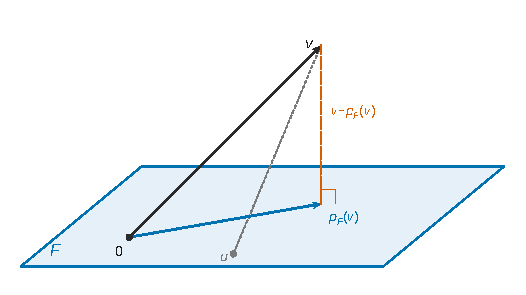
\includegraphics{figures/q3-projection-orthogonale.pdf}
\caption*{Figure 1 --- projection orthogonale sur F : p\_F(v) est le point de F le
plus proche de v, le résidu v − p\_F(v) est orthogonal à F et sa norme
est la distance de v à F (schéma, F hyperplan de ℳ₄,₁(ℝ))}
\end{figure}

\hypertarget{ii-suxe9ries-de-fourier}{%
\subsection{II --- Séries de Fourier}\label{ii-suxe9ries-de-fourier}}

\hypertarget{question-4}{%
\subsection{Question 4}\label{question-4}}

\emph{\(f\in E\).} Sur \(]-\pi,\pi]\), \(f\) coïncide avec \(t\mapsto\cos(\alpha t)\), continue. Au point \(-\pi\), on a
\equationajustee{\begin{aligned}
f(-\pi)&=f(\pi)=\cos(\alpha\pi),\\
\lim_{x\to-\pi^+}f(x)&=\cos(-\alpha\pi)=\cos(\alpha\pi).
\end{aligned}}
Donc \(f\) est continue sur \(\mathbb R\) et \(2\pi\)-périodique ; elle est de plus \(\mathcal C^1\) par morceaux.

\emph{Parité.} Pour \(x\in]-\pi,\pi[\), \(f(-x)=\cos(-\alpha x)=f(x)\), et \(f(-\pi)=f(\pi)\). Par périodicité, \(f\) est paire.

Pour \(n\geqslant1\), \(t\mapsto f(t)\sin(nt)\) est impaire et \(2\pi\)-périodique. L'intégrale sur une période ne dépendant pas de la période choisie,
\equationajustee{b_n(f)=\frac1\pi\int_{-\pi}^{\pi}f(t)\sin(nt)\,dt=0.}

\emph{Calcul de \(a_0\).} Comme \(\alpha\neq0\) :
\equationajustee{\begin{aligned}
a_0(f)&=\frac1{2\pi}\int_{-\pi}^{\pi}\cos(\alpha t)\,dt\\
&=\frac1{2\pi}\cdot\frac{2\sin(\alpha\pi)}{\alpha}\\
&=\frac{\sin(\alpha\pi)}{\alpha\pi}.
\end{aligned}}

\emph{Calcul de \(a_n\), \(n\geqslant1\).} On linéarise :
\equationajustee{\cos(\alpha t)\cos(nt)=\tfrac12\big[\cos((\alpha+n)t)+\cos((\alpha-n)t)\big].}
Comme \(\alpha\notin\mathbb Z\), on a \(\alpha\pm n\neq0\). De plus \(\sin((\alpha\pm n)\pi)=(-1)^n\sin(\alpha\pi)\), donc
\equationajustee{\begin{aligned}
a_n(f)&=\frac1{2\pi}\left[\frac{2\sin((\alpha+n)\pi)}{\alpha+n}+\frac{2\sin((\alpha-n)\pi)}{\alpha-n}\right]\\
&=\frac{(-1)^n\sin(\alpha\pi)}{\pi}\left(\frac1{\alpha+n}+\frac1{\alpha-n}\right).
\end{aligned}}
\equationajustee{\boxed{\begin{aligned}
b_n(f)&=0,\\
a_0(f)&=\frac{\sin(\alpha\pi)}{\alpha\pi},\\
a_n(f)&=\frac{(-1)^n}{\pi}\,\frac{2\alpha\sin(\alpha\pi)}{\alpha^2-n^2}.
\end{aligned}}}

\hypertarget{question-5}{%
\subsection{Question 5}\label{question-5}}

\emph{Convergence.} Comme \(\alpha\notin\mathbb Z\), les termes sont définis, et \(n^2-\alpha^2\sim n^2\). Donc
\equationajustee{\begin{aligned}
\left|\frac1{n^2-\alpha^2}\right|&\sim\frac1{n^2},\\
\frac1{(n^2-\alpha^2)^2}&\sim\frac1{n^4}.
\end{aligned}}
Par comparaison à des séries de Riemann convergentes, les deux séries convergent absolument.

\emph{Première somme.} \(f\) est continue, \(2\pi\)-périodique et \(\mathcal C^1\) par morceaux. Par le théorème de Dirichlet, \(S_N(f)(x)\to f(x)\) pour tout réel \(x\).

En \(x=\pi\), avec \(\cos(n\pi)=(-1)^n\) :
\equationajustee{\begin{aligned}
\cos(\alpha\pi)&=\frac{\sin(\alpha\pi)}{\alpha\pi}+\frac{2\alpha\sin(\alpha\pi)}{\pi}\sum_{n=1}^{+\infty}\frac{1}{\alpha^2-n^2}\\
&=\frac{\sin(\alpha\pi)}{\alpha\pi}-\frac{2\alpha\sin(\alpha\pi)}{\pi}\sum_{n=1}^{+\infty}\frac{1}{n^2-\alpha^2}.
\end{aligned}}
Comme \(\sin(\alpha\pi)\neq0\) :
\equationajustee{\boxed{\sum_{n=1}^{+\infty}\frac1{n^2-\alpha^2}=\frac1{2\alpha^2}-\frac{\pi\cos(\alpha\pi)}{2\alpha\sin(\alpha\pi)}.}}

\emph{Seconde somme.} La formule de Parseval s'applique à \(f\), continue par morceaux et \(2\pi\)-périodique :
\equationajustee{\frac1{2\pi}\int_0^{2\pi}f^2=a_0(f)^2+\frac12\sum_{n=1}^{+\infty}\big(a_n(f)^2+b_n(f)^2\big).}
D'une part, avec \(\cos^2(\alpha t)=\frac{1+\cos(2\alpha t)}2\),
\equationajustee{\begin{aligned}
\frac1{2\pi}\int_{-\pi}^{\pi}\cos^2(\alpha t)\,dt&=\frac12+\frac{\sin(2\alpha\pi)}{4\alpha\pi}\\
&=\frac12+\frac{\sin(\alpha\pi)\cos(\alpha\pi)}{2\alpha\pi}.
\end{aligned}}
D'autre part, notons \(S=\sum_{n\geqslant1}\frac1{(n^2-\alpha^2)^2}\). Puisque
\equationajustee{a_n(f)^2=\frac{4\alpha^2\sin^2(\alpha\pi)}{\pi^2(n^2-\alpha^2)^2},}
le membre de droite vaut
\equationajustee{\frac{\sin^2(\alpha\pi)}{\alpha^2\pi^2}+\frac{2\alpha^2\sin^2(\alpha\pi)}{\pi^2}S.}
D'où
\equationajustee{S=\frac{\pi^2}{2\alpha^2\sin^2(\alpha\pi)}\left[\frac12+\frac{\sin(\alpha\pi)\cos(\alpha\pi)}{2\alpha\pi}-\frac{\sin^2(\alpha\pi)}{\alpha^2\pi^2}\right],}
\equationajustee{\boxed{\sum_{n=1}^{+\infty}\frac1{(n^2-\alpha^2)^2}=\frac{\pi^2}{4\alpha^2\sin^2(\alpha\pi)}+\frac{\pi\cos(\alpha\pi)}{4\alpha^3\sin(\alpha\pi)}-\frac1{2\alpha^4}.}}
(Contrôle pour \(\alpha=0{,}3\) : \(1{,}751388\) et \(1{,}293131\).)

\hypertarget{question-6}{%
\subsection{Question 6}\label{question-6}}

Soit \(t\in\mathbb R\setminus\pi\mathbb Z\) et \(\alpha=t/\pi\in\mathbb R\setminus\mathbb Z\). La relation obtenue en \(x=\pi\) à la question 5, divisée par \(\sin(\alpha\pi)\neq0\) et multipliée par \(\pi\), s'écrit
\equationajustee{\frac{\pi\cos(\alpha\pi)}{\sin(\alpha\pi)}=\frac1\alpha+\sum_{n=1}^{+\infty}\frac{2\alpha}{\alpha^2-n^2}.}
Avec \(\alpha=t/\pi\), on a
\equationajustee{\begin{aligned}
\frac{2\alpha}{\alpha^2-n^2}&=\frac{2t\pi}{t^2-(n\pi)^2},\\
\frac1\alpha&=\frac\pi t.
\end{aligned}}
En divisant par \(\pi\) :
\equationajustee{\boxed{\frac{\cos t}{\sin t}=\frac1t+\sum_{n=1}^{+\infty}\frac{2t}{t^2-(n\pi)^2}.}}

\hypertarget{question-7}{%
\subsection{Question 7}\label{question-7}}

Soit \(n\in\mathbb N^*\). Par linéarité de l'intégrale et \(e^{\mp int}=\cos(nt)\mp i\sin(nt)\) :
\equationajustee{\begin{aligned}
c_n(f)&=\frac12\cdot\frac1\pi\int_0^{2\pi}f(t)\cos(nt)\,dt-\frac i2\cdot\frac1\pi\int_0^{2\pi}f(t)\sin(nt)\,dt\\
&=\frac{a_n(f)-ib_n(f)}2,
\end{aligned}}
\equationajustee{c_{-n}(f)=\frac1{2\pi}\int_0^{2\pi}f(t)e^{int}\,dt=\frac{a_n(f)+ib_n(f)}2.}
En additionnant : \(c_n(f)+c_{-n}(f)=a_n(f)\).

En soustrayant : \(c_n(f)-c_{-n}(f)=-ib_n(f)\), puis on multiplie par \(i\) :
\equationajustee{\boxed{\begin{aligned}
a_n(f)&=c_n(f)+c_{-n}(f),\\
b_n(f)&=i\big(c_n(f)-c_{-n}(f)\big).
\end{aligned}}}

\hypertarget{question-8}{%
\subsection{Question 8}\label{question-8}}

Soit \(n\in\mathbb Z\). La fonction \(f\) est \(\mathcal C^2\) et \(2\pi\)-périodique. Donc \(f(2\pi)=f(0)\) et \(f'(2\pi)=f'(0)\).

De plus \(e^{-2in\pi}=1\). Deux intégrations par parties donnent
\equationajustee{\begin{aligned}
\int_0^{2\pi}f''(t)e^{-int}dt&=\big[f'(t)e^{-int}\big]_0^{2\pi}+in\int_0^{2\pi}f'(t)e^{-int}dt\\
&=in\Big(\big[f(t)e^{-int}\big]_0^{2\pi}+in\int_0^{2\pi}f(t)e^{-int}dt\Big),
\end{aligned}}
les crochets étant nuls. Donc \(c_n(f'')=(in)^2c_n(f)=-n^2c_n(f)\).

Par \((\mathcal E)\), \(f''(t)=-e^{it}f(t)\), donc
\equationajustee{c_n(f'')=-\frac1{2\pi}\int_0^{2\pi}f(t)e^{-i(n-1)t}dt=-c_{n-1}(f).}
En comparant : \(\boxed{c_{n-1}(f)=n^2c_n(f)}\) pour tout \(n\in\mathbb Z\).

\emph{Indices négatifs.} Pour \(n=0\), on obtient \(c_{-1}(f)=0\). Supposons \(c_{-k}(f)=0\) pour un \(k\geqslant1\). La relation en \(n=-k\) donne alors
\equationajustee{c_{-k-1}(f)=k^2c_{-k}(f)=0.}
Par récurrence, \(c_n(f)=0\) pour tout \(n<0\).

\emph{Indices positifs.} Pour \(n\geqslant1\), \(c_n(f)=\frac{c_{n-1}(f)}{n^2}\). Par récurrence (vrai en \(n=0\)), et puisque \(n!=n\,(n-1)!\), on obtient \(c_n(f)=\frac{c_0(f)}{(n!)^2}\).
\equationajustee{\boxed{c_n(f)=\begin{cases}\dfrac{c_0(f)}{(n!)^2}&\text{si }n\geqslant0\\[2mm]0&\text{si }n<0.\end{cases}}}

\hypertarget{question-9}{%
\subsection{Question 9}\label{question-9}}

Posons \(u=\operatorname{Re}f\) et \(v=\operatorname{Im}f\). Ces fonctions réelles sont \(2\pi\)-périodiques et de classe \(\mathcal C^2\), donc continues et \(\mathcal C^1\) par morceaux.

Par le théorème de Dirichlet, \(S_N(u)(x)\to u(x)\) et \(S_N(v)(x)\to v(x)\) pour tout \(x\). Par linéarité des coefficients, \(S_N(f)=S_N(u)+iS_N(v)\), qui converge simplement vers \(f\).

Par Q7, pour \(n\geqslant1\),
\equationajustee{\begin{aligned}
a_n(f)\cos(nx)+b_n(f)\sin(nx)&=(c_n+c_{-n})\cos(nx)+i(c_n-c_{-n})\sin(nx)\\
&=c_n(f)e^{inx}+c_{-n}(f)e^{-inx},
\end{aligned}}
et \(a_0(f)=c_0(f)\). Donc
\equationajustee{S_N(f)(x)=c_0(f)+\sum_{n=1}^N\big(c_n(f)e^{inx}+c_{-n}(f)e^{-inx}\big).}
En passant à la limite puis en utilisant Q8 :
\equationajustee{\boxed{\begin{aligned}
f(x)&=c_0(f)+\sum_{n=1}^{+\infty}\big(c_n(f)e^{inx}+c_{-n}(f)e^{-inx}\big)\\
&=c_0(f)\sum_{n=0}^{+\infty}\frac{e^{inx}}{(n!)^2}.
\end{aligned}}}
(La série converge absolument car \(\sum\frac1{(n!)^2}\) converge.)

\hypertarget{question-10}{%
\subsection{Question 10}\label{question-10}}

\emph{Dimension.} L'équation \((\mathcal E)\) s'écrit \(y''+a(x)y'+b(x)y=0\). Les coefficients \(a=0\) et \(b:x\mapsto e^{ix}\) sont continus sur l'intervalle \(\mathbb R\).

Par le théorème de Cauchy linéaire, pour tout \((\mu,\nu)\in\mathbb C^2\), il existe une unique solution \(g\) telle que \(g(0)=\mu\) et \(g'(0)=\nu\).

L'application linéaire \(g\mapsto(g(0),g'(0))\) est donc un isomorphisme de l'espace \(\mathcal S\) des solutions sur \(\mathbb C^2\) :
\equationajustee{\boxed{\dim_{\mathbb C}\mathcal S=2.}}

\emph{Solutions non périodiques.} Soit \(g_0:x\mapsto\sum_{n\geqslant0}\frac{e^{inx}}{(n!)^2}\), solution admise. Elle est \(2\pi\)-périodique et non nulle, car \(g_0(0)=\sum\frac1{(n!)^2}>0\).

Soit \(\mathcal P\) le sous-espace des solutions \(2\pi\)-périodiques. Toute \(g\in\mathcal P\) est \(\mathcal C^2\) et \(2\pi\)-périodique, donc Q9 donne \(g=c_0(g)g_0\).

Ainsi \(\mathcal P=\mathbb Cg_0\) est de dimension 1.

Comme \(\dim\mathcal S=2>1\), il existe des solutions non \(2\pi\)-périodiques.

Par exemple, soit \(g_1\) la solution telle que \(g_1(0)=0\) et \(g_1'(0)=1\).

Si elle valait \(cg_0\), alors \(cg_0(0)=0\) imposerait \(c=0\). On aurait \(g_1=0\), ce qui contredit \(g_1'(0)=1\).

\textbf{Oui, \((\mathcal E)\) admet des solutions qui ne sont pas \(2\pi\)-périodiques.}

\hypertarget{question-11}{%
\subsection{Question 11}\label{question-11}}

Toutes ces fonctions sont dans \(E\). Pour \(n\neq m\) dans \(\mathbb N\), les entiers \(n+m\) et \(n-m\) sont non nuls.

Or \(\int_0^{2\pi}\cos(kx)\,dx=0\) pour \(k\in\mathbb Z^*\), donc
\equationajustee{\varphi(e_n,e_m)=\frac1{4\pi}\int_0^{2\pi}\big[\cos((n+m)x)+\cos((n-m)x)\big]dx=0.}
De même, pour \(1\leqslant n\neq m\),
\equationajustee{\varphi(f_n,f_m)=\frac1{4\pi}\int_0^{2\pi}\big[\cos((n-m)x)-\cos((n+m)x)\big]dx=0.}
Soient \(n\in[\![0,N]\!]\) et \(m\in[\![1,N]\!]\). Comme \(\int_0^{2\pi}\sin(kx)\,dx=0\) pour tout \(k\in\mathbb Z\),
\equationajustee{\varphi(e_n,f_m)=\frac1{4\pi}\int_0^{2\pi}\big[\sin((n+m)x)-\sin((n-m)x)\big]dx=0.}
La famille est orthogonale. Elle n'est pas orthonormale : \(\|e_0\|^2=1\), mais pour \(n\geqslant1\),
\equationajustee{\|e_n\|^2=\frac1{4\pi}\int_0^{2\pi}(1+\cos(2nx))\,dx=\frac12,}
et de même \(\|f_n\|^2=\frac12\).
\textbf{La famille est orthogonale, non orthonormale :}
\equationajustee{\boxed{\begin{aligned}{}&\|e_0\|=1,\\
&\|e_n\|=\|f_n\|=\tfrac1{\sqrt2}\quad(n\geqslant1).
\end{aligned}}}

\hypertarget{question-12}{%
\subsection{Question 12}\label{question-12}}

D'après Q11, \((e_0,\dots,e_N,f_1,\dots,f_N)\) est une base orthogonale de \(V_N\) (vecteurs non nuls orthogonaux, générateurs par définition). Donc
\equationajustee{p_{V_N}(g)=\frac{\varphi(g,e_0)}{\|e_0\|^2}e_0+\sum_{n=1}^N\left(\frac{\varphi(g,e_n)}{\|e_n\|^2}e_n+\frac{\varphi(g,f_n)}{\|f_n\|^2}f_n\right).}
Or, pour \(n\geqslant1\),
\equationajustee{\begin{aligned}
\frac{\varphi(g,e_0)}{1}&=a_0(g),\\
\frac{\varphi(g,e_n)}{1/2}&=\frac1\pi\int_0^{2\pi}g(t)\cos(nt)\,dt=a_n(g),\\
\frac{\varphi(g,f_n)}{1/2}&=b_n(g).
\end{aligned}}
\equationajustee{\boxed{\begin{aligned}
p_{V_N}(g)&=a_0(g)+\sum_{n=1}^N\big(a_n(g)e_n+b_n(g)f_n\big)\\
&=S_N(g).
\end{aligned}}}
\(V_N\) étant de dimension finie, le projeté orthogonal est l'unique élément de \(V_N\) qui minimise la distance à \(g\). Ainsi \textbf{\(h=S_N(g)\in E\) vérifie \(\|g-h\|=\min_{v\in V_N}\|g-v\|\)}.

\hypertarget{partie-b-limites-de-suites-de-matrices}{%
\section{Partie B --- Limites de suites de matrices}\label{partie-b-limites-de-suites-de-matrices}}

\hypertarget{question-13}{%
\subsection{Question 13}\label{question-13}}

\emph{Cas de \(A\).} On a \(A^2=I_2\). Donc \(A^{2k}=I_2\) et \(A^{2k+1}=A\).

Supposons que \((A^k)\) converge vers \(L\). Les suites extraites \((A^{2k})\) et \((A^{2k+1})\) convergent aussi vers \(L\) (coefficient par coefficient).

On a alors \(L=I_2\) et \(L=A\), ce qui est absurde puisque \(A\neq I_2\). Donc \((A^k)\) diverge.

\emph{Cas de \(B\).} Avec \(\theta=\frac{2\pi}3\),
\equationajustee{B=\begin{pmatrix}\cos\theta&-\sin\theta\\\sin\theta&\cos\theta\end{pmatrix}.}
Par récurrence, grâce aux formules d'addition,
\equationajustee{B^k=\begin{pmatrix}\cos k\theta&-\sin k\theta\\\sin k\theta&\cos k\theta\end{pmatrix}.}
Donc \(B^3=I_2\), d'où \(B^{3k}=I_2\) et \(B^{3k+1}=B\). Le même raisonnement donne \(I_2=B\), ce qui est absurde.
\equationajustee{\boxed{(A^k)_{k\in\mathbb N}\text{ et }(B^k)_{k\in\mathbb N}\text{ divergent.}}}

\hypertarget{question-14}{%
\subsection{Question 14}\label{question-14}}

Soit \(A=PDP^{-1}\) avec \(P\in GL_n(\mathbb R)\) et \(D=\operatorname{Diag}(\mu_1,\dots,\mu_n)\) réelle. Alors \(\operatorname{Sp}(A)=\{\mu_1,\dots,\mu_n\}\subset\mathbb R\) et
\equationajustee{\begin{aligned}
A^k&=PD^kP^{-1},\\
D^k&=\operatorname{Diag}(\mu_1^k,\dots,\mu_n^k).
\end{aligned}}

\emph{Lemme.} Pour \(\mu\in\mathbb R\), \((\mu^k)\) converge si et seulement si \(\mu\in]-1,1]\). En effet :
- si \(|\mu|<1\), \(\mu^k\to0\) ;
- si \(\mu=1\), la suite est constante ;
- si \(\mu=-1\), elle vaut alternativement \(1\) et \(-1\) ;
- si \(|\mu|>1\), elle n'est pas bornée.

\emph{Sens direct.} Supposons que \((A^k)\) converge. Par le résultat admis (avec \(P^{-1}\) à gauche et \(P\) à droite), \((D^k)=(P^{-1}A^kP)\) converge. Donc chaque \((\mu_i^k)\) converge et \(\mu_i\in]-1,1]\).

\emph{Réciproque.} Si \(\operatorname{Sp}(A)\subset]-1,1]\), chaque \((\mu_i^k)\) converge, donc \((D^k)\) converge (coefficients non diagonaux nuls). Puis \((PD^kP^{-1})=(A^k)\) converge.
\equationajustee{\boxed{(A^k)\text{ converge}\iff\operatorname{Sp}(A)\subset]-1,1].}}

\hypertarget{question-15}{%
\subsection{Question 15}\label{question-15}}

\(A\) est symétrique réelle, donc diagonalisable sur \(\mathbb R\) (théorème spectral).

Plus précisément, soit \(J\) la matrice dont tous les coefficients valent 1 : \(2A=J-I_3\).
- Pour \(w=(1,1,1)^T\), \(Jw=3w\), donc \(Aw=w\).
- Pour \(x\) dans le plan \(H=\{x_1+x_2+x_3=0\}\), \(Jx=0\), donc \(Ax=-\frac12x\).

Comme \(\dim H=2\) et \(w\notin H\), on a \(\mathcal M_{3,1}(\mathbb R)=\mathbb Rw\oplus H\). C'est une somme de sous-espaces propres, ce qui redonne la diagonalisabilité. Enfin \(\operatorname{Sp}(A)=\{1,-\frac12\}\subset]-1,1]\). Par Q14 :
\equationajustee{\boxed{A\text{ est diagonalisable sur }\mathbb R\text{ et }(A^k)\text{ converge.}}}
(Sa limite est le projecteur sur \(\mathbb Rw\) parallèlement à \(H\), soit \(\frac13J\).)

\hypertarget{question-16}{%
\subsection{Question 16}\label{question-16}}

Pour \(x=(x_1,x_2,x_3)^T\), \(Ax=(x_2,x_3,x_1+x_2-x_3)^T\). La lecture des colonnes de \(T\) conduit à chercher \(u,v,w\) avec
\equationajustee{\begin{aligned}
Au&=u,\\
Av&=-v,\\
Aw&=v-w.
\end{aligned}}

\begin{itemize}
\tightlist
\item
  \(Au=u\) : \(u_2=u_1\), \(u_3=u_2\), la troisième équation suit ; \(u=(1,1,1)^T\).
\item
  \(Av=-v\) : \(v_2=-v_1\), \(v_3=-v_2\), la troisième suit ; \(v=(1,-1,1)^T\).
\item
  \((A+I_3)w=v\) : \(w_1+w_2=1\), \(w_2+w_3=-1\) (la troisième équation répète la première) ; \(w=(1,0,-1)^T\).
\end{itemize}

Soit
\equationajustee{P=\begin{pmatrix}1&1&1\\1&-1&0\\1&1&-1\end{pmatrix}.}
On a \(\det P=1\cdot1-1\cdot(-1)+1\cdot2=4\neq0\), donc \(P\) est inversible. Par construction,
\equationajustee{AP=\begin{pmatrix}1&-1&0\\1&1&-1\\1&-1&2\end{pmatrix}=PT.}
Donc
\equationajustee{\boxed{A=PTP^{-1}:\ A\text{ et }T\text{ sont semblables.}}}

\emph{Convergence.} Considérons le bloc
\equationajustee{N=\begin{pmatrix}-1&1\\0&-1\end{pmatrix}=-I_2+F,}
où
\equationajustee{F=\begin{pmatrix}0&1\\0&0\end{pmatrix}.}
On a \(F^2=0\), et \(-I_2\) commute avec \(F\). Par la formule du binôme, \(N^k=(-1)^kI_2+k(-1)^{k-1}F\), donc
\equationajustee{T^k=\begin{pmatrix}1&0&0\\0&(-1)^k&(-1)^{k-1}k\\0&0&(-1)^k\end{pmatrix}.}
Le coefficient \((2,3)\) n'est pas borné : \((T^k)\) diverge. Si \((A^k)\) convergeait, \((P^{-1}A^kP)=(T^k)\) convergerait (résultat admis). Donc \textbf{\((A^k)\) diverge}.

(Q14 ne s'applique pas : \(A+I_3\) est de rang 2, donc \(A\) n'est pas diagonalisable.)

\hypertarget{partie-c-interpolation-polynuxf4miale-et-moindres-carruxe9s}{%
\section{Partie C --- Interpolation polynômiale et moindres carrés}\label{partie-c-interpolation-polynuxf4miale-et-moindres-carruxe9s}}

\hypertarget{question-17}{%
\subsection{Question 17}\label{question-17}}

Les \(x_j\) étant distincts, les dénominateurs sont non nuls et \(L_i\in\mathbb R_n[X]\) (degré \(n\)).

Si \(k\neq i\), le facteur d'indice \(j=k\) vaut \(\frac{x_k-x_k}{x_i-x_k}=0\). Si \(k=i\), chaque facteur vaut \(1\).
\equationajustee{\boxed{L_i(x_k)=\begin{cases}1&\text{si }k=i\\0&\text{sinon.}\end{cases}}}

\hypertarget{question-18}{%
\subsection{Question 18}\label{question-18}}

L'application est symétrique. Elle est linéaire à gauche, car \((\lambda P+P')(x_k)=\lambda P(x_k)+P'(x_k)\), donc bilinéaire. Elle est positive : \(\langle P,P\rangle=\sum_kP(x_k)^2\geqslant0\).

Si \(\langle P,P\rangle=0\), chaque \(P(x_k)\) est nul. Alors \(P\) admet \(n+1\) racines distinctes.

Comme \(\deg P\leqslant n\), on obtient \(P=0\). \textbf{C'est un produit scalaire sur \(\mathbb R_n[X]\).}

\hypertarget{question-19}{%
\subsection{Question 19}\label{question-19}}

Par Q17, la somme \(\langle L_i,L_j\rangle=\sum_kL_i(x_k)L_j(x_k)\) n'a au plus qu'un terme non nul, celui où \(k=i=j\), qui vaut 1. Donc \(\langle L_i,L_j\rangle=\delta_{ij}\) : la famille est orthonormée, donc libre.

Elle a \(n+1=\dim\mathbb R_n[X]\) éléments, c'est donc une base. \textbf{\((L_0,\dots,L_n)\) est une base orthonormée de \(\mathbb R_n[X]\).}

\hypertarget{question-20}{%
\subsection{Question 20}\label{question-20}}

Par Q17, \(\langle L_i,P\rangle=\sum_kL_i(x_k)P(x_k)=P(x_i)\). La décomposition dans la base orthonormée \((L_i)\) donne
\equationajustee{\boxed{\begin{aligned}
\langle L_i,P\rangle&=P(x_i),\\
P&=\sum_{i=0}^n\langle L_i,P\rangle L_i=\sum_{i=0}^nP(x_i)L_i.
\end{aligned}}}
En particulier \(P_f(x_k)=f(x_k)\) pour tout \(k\).

\hypertarget{question-21}{%
\subsection{Question 21}\label{question-21}}

Comme \(m\leqslant n\), \(\mathbb R_m[X]\) est un sous-espace de \(\mathbb R_n[X]\), de dimension finie. Pour \(Q\in\mathbb R_m[X]\), puisque \(P_f(x_i)=f(x_i)\),
\equationajustee{\begin{aligned}
\langle P_f-Q,P_f-Q\rangle&=\sum_{i=0}^n\big(P_f(x_i)-Q(x_i)\big)^2\\
&=\sum_{i=0}^n\big(f(x_i)-Q(x_i)\big)^2.
\end{aligned}}
Minimiser cette somme revient donc à minimiser \(\|P_f-Q\|\) sur \(\mathbb R_m[X]\). D'après le théorème de la projection orthogonale, ce minimum est atteint en un unique point, \(R=p_{\mathbb R_m[X]}(P_f)\).

\textbf{Il existe un unique \(R\in\mathbb R_m[X]\) tel que}
\equationajustee{\boxed{\begin{aligned}{}&\sum_{i=0}^n(f(x_i)-R(x_i))^2\\
={}&\min_{Q\in\mathbb R_m[X]}\sum_{i=0}^n(f(x_i)-Q(x_i))^2,
\end{aligned}}}
\textbf{à savoir \(R=p_{\mathbb R_m[X]}(P_f)\).}

\hypertarget{question-22}{%
\subsection{Question 22}\label{question-22}}

Pour \(n\in\mathbb N\), notons \(H_n\) la propriété suivante. Pour toute fonction \(g\in\mathcal C^{n+1}([a,b],\mathbb R)\) ayant au moins \(n+2\) zéros distincts, la dérivée \(g^{(n+1)}\) s'annule sur \([a,b]\).

\emph{\(H_0\).} Soit \(g\in\mathcal C^1\) qui s'annule en \(c<d\). Le théorème de Rolle sur \([c,d]\) donne un zéro de \(g'\).

\emph{\(H_n\Rightarrow H_{n+1}\).} Soit \(g\in\mathcal C^{n+2}([a,b])\) ayant des zéros \(c_0<\dots<c_{n+2}\).

Pour \(j\in[\![0,n+1]\!]\), Rolle sur \([c_j,c_{j+1}]\) donne \(d_j\in]c_j,c_{j+1}[\) avec \(g'(d_j)=0\).

Les intervalles étant disjoints, \(g'\in\mathcal C^{n+1}\) a \(n+2\) zéros distincts. \(H_n\) appliquée à \(g'\) fournit un zéro de \(g^{(n+2)}\).

\textbf{Par récurrence, \(H_n\) est vraie pour tout \(n\) : \(g^{(n+1)}\) s'annule au moins une fois sur \([a,b]\).}

\begin{figure}[H]
\centering
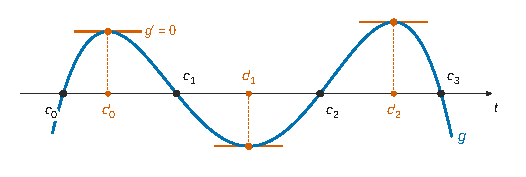
\includegraphics{figures/q22-rolle-zeros.pdf}
\caption*{Figure 2 --- Rolle entre zéros consécutifs : entre c\_j et c\_\{j+1\}, g
a une tangente horizontale en d\_j, zéro de g′ ; quatre zéros de g
donnent trois zéros distincts de g′}
\end{figure}

\hypertarget{question-23}{%
\subsection{Question 23}\label{question-23}}

\(K\) est défini car \(x\neq x_i\) pour tout \(i\).

\(W\) est de classe \(\mathcal C^{n+1}\) sur \([a,b]\). Pour tout \(k\), et au point \(x\),
\equationajustee{\begin{aligned}
W(x_k)&=f(x_k)-P_f(x_k)-0=0,\\
W(x)&=f(x)-P_f(x)-(f(x)-P_f(x))=0.
\end{aligned}}
Les points \(x_0,\dots,x_n,x\) sont \(n+2\) points distincts de \([a,b]\) où \(W\) s'annule.

Par Q22, il existe \(\xi_x\in[a,b]\) avec \(W^{(n+1)}(\xi_x)=0\). Or \(\deg P_f\leqslant n\) donne \(P_f^{(n+1)}=0\).

Et \(\prod_i(t-x_i)\) est unitaire de degré \(n+1\), de dérivée \((n+1)\)-ième égale à \((n+1)!\). Donc
\equationajustee{W^{(n+1)}(t)=f^{(n+1)}(t)-K(n+1)!,}
d'où \(K=\frac{f^{(n+1)}(\xi_x)}{(n+1)!}\) et
\equationajustee{\boxed{f(x)-P_f(x)=\frac{\prod_{i=0}^n(x-x_i)}{(n+1)!}f^{(n+1)}(\xi_x).}}

\hypertarget{partie-d-ruxe9gression-linuxe9aire-et-moindres-carruxe9s}{%
\section{Partie D --- Régression linéaire et moindres carrés}\label{partie-d-ruxe9gression-linuxe9aire-et-moindres-carruxe9s}}

\hypertarget{i-le-cas-particulier-de-la-dimension-2}{%
\subsection{I --- Le cas particulier de la dimension 2}\label{i-le-cas-particulier-de-la-dimension-2}}

\hypertarget{question-24}{%
\subsection{Question 24}\label{question-24}}

La \(i\)-ème composante de \(A\binom ab-Y\) est \(a+bx_i-y_i\), donc
\equationajustee{E(a,b)=\left\|A\binom ab-Y\right\|_2^2.}
Quand \((a,b)\) décrit \(\mathbb R^2\), le vecteur \(A\binom ab=aC_1+bC_2\) décrit \(\operatorname{Col}(A)\). C'est un sous-espace de dimension finie de \(\mathcal M_{n,1}(\mathbb R)\).

Le projeté \(z_0=p_{\operatorname{Col}(A)}(Y)\) s'écrit \(A\binom{a_0}{b_0}\).

Il vérifie \(\|z_0-Y\|_2\leqslant\|z-Y\|_2\) pour tout \(z\in\operatorname{Col}(A)\). Donc \(E(a_0,b_0)\leqslant E(a,b)\) pour tout \((a,b)\) : \(E\) admet un minimum et
\equationajustee{\boxed{\begin{aligned}
m&=\min_{(a,b)\in\mathbb R^2}E(a,b)\\
&=\min_{(a,b)\in\mathbb R^2}\left\|A\begin{pmatrix}a\\b\end{pmatrix}-Y\right\|_2^2\\
&=\big\|Y-p_{\operatorname{Col}(A)}(Y)\big\|_2^2.
\end{aligned}}}

\hypertarget{question-25}{%
\subsection{Question 25}\label{question-25}}

\equationajustee{A^TA=\begin{pmatrix}n&\sum x_k\\\sum x_k&\sum x_k^2\end{pmatrix},}
\equationajustee{\boxed{\det(A^TA)=n\sum_{1\leqslant k\leqslant n}x_k^2-\Big(\sum_{1\leqslant k\leqslant n}x_k\Big)^2.}}
Posons \(X=(x_1,\dots,x_n)\) et \(U=(1,\dots,1)\). L'inégalité de Cauchy-Schwarz donne \(\langle X,U\rangle^2\leqslant\|X\|^2\|U\|^2\), soit \((\sum x_k)^2\leqslant n\sum x_k^2\). Il y a égalité si et seulement si \((X,U)\) est liée. L'hypothèse de non-colinéarité rend l'inégalité stricte : \(\boxed{\det(A^TA)>0.}\)

\hypertarget{question-26}{%
\subsection{Question 26}\label{question-26}}

\(E\) est polynomiale, donc \(\mathcal C^1\) sur \(\mathbb R^2\), et
\equationajustee{\begin{aligned}
\frac{\partial E}{\partial a}&=-2\sum_{i=1}^n(y_i-a-bx_i),\\
\frac{\partial E}{\partial b}&=-2\sum_{i=1}^nx_i(y_i-a-bx_i),
\end{aligned}}
\equationajustee{\boxed{\nabla E(a,b)=2\left(A^TA\begin{pmatrix}a\\b\end{pmatrix}-A^TY\right).}}
Un point critique \((a_0,b_0)\) vérifie donc \(\boxed{A^TA\binom{a_0}{b_0}=A^TY.}\)

Par Q25, \(A^TA\) est inversible : il y a au plus un point critique, \((A^TA)^{-1}A^TY\).

Par Q24, \(E\) atteint son minimum en un point \((c,d)\). \(\mathbb R^2\) étant ouvert et \(E\) de classe \(\mathcal C^1\), \((c,d)\) est un point critique. Tout point de minimum est donc égal à l'unique point critique.

\textbf{Il existe un unique \((c,d)\in\mathbb R^2\) tel que \(E(c,d)=\min E\), à savoir \(\binom cd=(A^TA)^{-1}A^TY\).}

\begin{figure}[H]
\centering
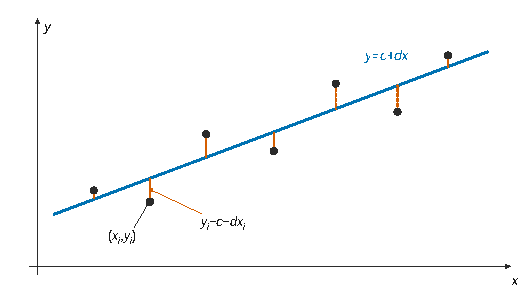
\includegraphics{figures/q26-droite-regression.pdf}
\caption*{Figure 3 --- droite des moindres carrés y = c + dx : E(c, d) est la
somme des carrés des écarts verticaux y\_i − c − dx\_i (tirets), non des
distances à la droite}
\end{figure}

\hypertarget{ii-les-moindres-carruxe9s-le-cas-guxe9nuxe9ral}{%
\subsection{II --- Les moindres carrés : le cas général}\label{ii-les-moindres-carruxe9s-le-cas-guxe9nuxe9ral}}

\hypertarget{question-27}{%
\subsection{Question 27}\label{question-27}}

On a
\equationajustee{\begin{aligned}
\|Ax\|_2^2&=(Ax)^T(Ax)\\
&=x^T(A^TAx)\\
&=0,
\end{aligned}}
donc \(\boxed{\|Ax\|_2=0.}\)

\hypertarget{question-28}{%
\subsection{Question 28}\label{question-28}}

Si \(Ax=0\), alors \(A^TAx=0\). Si \(A^TAx=0\), alors \(\|Ax\|_2=0\) (Q27), donc \(Ax=0\). Ainsi \(\ker(A^TA)=\ker A\).

Les deux matrices définissent des applications linéaires de source \(\mathcal M_{p,1}(\mathbb R)\). Le théorème du rang donne
\equationajustee{\begin{aligned}
\operatorname{rg}(A)&=p-\dim\ker A\\
&=p-\dim\ker(A^TA)\\
&=\operatorname{rg}(A^TA).
\end{aligned}}
\equationajustee{\boxed{\begin{aligned}
\ker(A^TA)&=\ker(A),\\
\operatorname{rg}(A^TA)&=\operatorname{rg}(A).
\end{aligned}}}

\hypertarget{question-29}{%
\subsection{Question 29}\label{question-29}}

\(\operatorname{Col}(A)\) est de dimension finie, donc \(\mathcal M_{n,1}(\mathbb R)=\operatorname{Col}(A)\oplus\operatorname{Col}(A)^\perp\). On a donc, de manière unique, \(y=z+d\) avec \(z=p_{\operatorname{Col}(A)}(y)\) et \(d\in\operatorname{Col}(A)^\perp\).

Comme \(Ax=\sum_jx_jC_j\), on a \(\operatorname{Col}(A)=\operatorname{Im}(A)\). Il existe donc \(u\) avec \(Au=z\), d'où \(y=Au+d\).

Soit \(y=Au'+d'\) une autre décomposition du même type. L'unicité de la décomposition dans la somme directe donne \(Au'=Au\) et \(d'=d\).

\textbf{Le vecteur \(d\) et le vecteur \(Au=p_{\operatorname{Col}(A)}(y)\) sont uniques ; \(u\) est unique à un élément de \(\ker A\) près.}

\emph{Remarque sur l'énoncé.} L'unicité de \(u\) lui-même n'a lieu que si \(\ker A=\{0\}\) : sinon \((u+h,d)\) convient pour tout \(h\in\ker A\). C'est cohérent avec Q30, et seules l'existence et l'unicité de \(d\) servent dans la suite.

\hypertarget{question-30}{%
\subsection{Question 30}\label{question-30}}

On écrit \(Ax-y=A(x-u)-d\), avec \(A(x-u)\in\operatorname{Col}(A)\) et \(d\in\operatorname{Col}(A)^\perp\). Par Pythagore,
\equationajustee{\begin{aligned}
\|Ax-y\|_2^2&=\|A(x-u)\|_2^2+\|d\|_2^2\\
&\geqslant\|d\|_2^2,
\end{aligned}}
avec égalité si et seulement si \(A(x-u)=0\).
\equationajustee{\boxed{\|Ax-y\|_2\geqslant\|d\|_2,\ \text{avec \text{égalité} si et seulement si } x-u\in\ker A.}}
En particulier \(\min_x\|Ax-y\|_2\) existe et vaut \(\|d\|_2\).

\hypertarget{question-31}{%
\subsection{Question 31}\label{question-31}}

\(d\) est orthogonal à chaque colonne \(C_j\). Or la \(j\)-ème composante de \(A^Td\) est \(C_j^Td=0\). Donc \(A^Td=0\).

En multipliant \(y=Au+d\) par \(A^T\) : \(\boxed{A^Ty=A^TAu.}\)

\hypertarget{question-32}{%
\subsection{Question 32}\label{question-32}}

Par Q30, \(\|Ax_0-y\|_2=\min\|Ax-y\|_2\) équivaut à \(x_0-u\in\ker A\). Par Q28 puis Q31,
\equationajustee{\begin{aligned}
x_0-u\in\ker A&\iff A^TA(x_0-u)=0\\
&\iff A^TAx_0=A^TAu\\
&\iff A^TAx_0=A^Ty.
\end{aligned}}
\equationajustee{\boxed{\begin{aligned}{}&\|Ax_0-y\|_2=\min_{x}\|Ax-y\|_2\\
\iff{}&A^TAx_0=A^Ty.
\end{aligned}}}

\hypertarget{question-33}{%
\subsection{Question 33}\label{question-33}}

Par Q28, \(\operatorname{rg}(A^TA)=\operatorname{rg}A=p\). Comme \(A^TA\) est carrée d'ordre \(p\), elle est \textbf{inversible}.

Par Q32, \(b\) réalise le minimum si et seulement si \(A^TAb=A^Ty\), c'est-à-dire
\equationajustee{\boxed{b=(A^TA)^{-1}A^Ty,}}
qui est donc l'unique solution.

\hypertarget{iii-la-duxe9composition-en-valeurs-singuliuxe8res}{%
\subsection{III --- La décomposition en valeurs singulières}\label{iii-la-duxe9composition-en-valeurs-singuliuxe8res}}

\hypertarget{question-34}{%
\subsection{Question 34}\label{question-34}}

On a
\equationajustee{\begin{aligned}
X^TA^TAX&=(AX)^T(AX)=\|AX\|_2^2\geqslant0,\\
X^TX&=\|X\|_2^2\geqslant0.
\end{aligned}}

\hypertarget{question-35}{%
\subsection{Question 35}\label{question-35}}

\((A^TA)^T=A^TA\) : la matrice est symétrique réelle. Par le théorème spectral, elle est semblable à une matrice diagonale réelle via une matrice orthogonale réelle. Ses valeurs propres sont réelles et admettent des vecteurs propres réels.

Soit \(A^TAX=\lambda X\) avec \(X\in\mathcal M_{p,1}(\mathbb R)\) non nul. Alors, par Q34,
\equationajustee{\|AX\|_2^2=X^TA^TAX=\lambda\|X\|_2^2,}
d'où \(\lambda=\frac{\|AX\|_2^2}{\|X\|_2^2}\geqslant0\). \textbf{Toutes les valeurs propres de \(A^TA\) sont positives ou nulles.}

\hypertarget{question-36}{%
\subsection{Question 36}\label{question-36}}

Par le théorème spectral, \(A^TA=WD_0W^T\) avec \(W\in O_p(\mathbb R)\) et \(D_0=\operatorname{Diag}(\mu_1,\dots,\mu_p)\), où \(\mu_i\geqslant0\) (Q35).

\(W\) étant inversible, \(\operatorname{rg}D_0=\operatorname{rg}(A^TA)=r\). Exactement \(r\) des \(\mu_i\) sont donc non nuls.

Soit \(P_\sigma\) la matrice de permutation qui range les \(\mu_i\) par ordre décroissant ; elle est orthogonale. On a
\equationajustee{P_\sigma^TD_0P_\sigma=\operatorname{Diag}(\lambda_1,\dots,\lambda_r,0,\dots,0),}
avec \(\lambda_1\geqslant\dots\geqslant\lambda_r>0\). Avec \(V=WP_\sigma\in O_p(\mathbb R)\) :
\equationajustee{\boxed{A^TA=V\operatorname{Diag}_{p,p}(\lambda_1,\dots,\lambda_r,0,\dots,0)V^T.}}
(\(r\geqslant1\) car \(A\neq0\).)

\hypertarget{question-37}{%
\subsection{Question 37}\label{question-37}}

Posons \(\lambda_i=0\) pour \(i>r\). De \(A^TAV=V\operatorname{Diag}(\lambda_i)\) on tire \(A^TAv_i=\lambda_iv_i\), et \(v_i^Tv_j=\delta_{ij}\). Donc
\equationajustee{\langle Av_i,Av_j\rangle=v_i^T(A^TAv_j)=\lambda_j\delta_{ij}.}
La famille \((Av_1,\dots,Av_r)\) est orthogonale et \(\|Av_i\|_2^2=\lambda_i\) :
\equationajustee{\boxed{\|Av_i\|_2=\begin{cases}\sqrt{\lambda_i}&\text{si }i\leqslant r\\0&\text{si }i\geqslant r+1.\end{cases}}}
Pour \(i\leqslant r\), \(u_i=\frac1{\sqrt{\lambda_i}}Av_i\) est bien défini, et
\equationajustee{\langle u_i,u_j\rangle=\frac{\lambda_j\delta_{ij}}{\sqrt{\lambda_i\lambda_j}}=\delta_{ij}.}
Ainsi \((u_1,\dots,u_r)\) est orthonormée. Soit \(G=\operatorname{Vect}(u_1,\dots,u_r)\) ; \(G^\perp\), de dimension \(n-r\), admet une base orthonormée \((u_{r+1},\dots,u_n)\).

\textbf{La famille \((u_1,\dots,u_n)\) est orthonormée de cardinal \(n\) : c'est une base orthonormée de \(\mathcal M_{n,1}(\mathbb R)\). Elle vérifie \(u_i=\frac1{\sqrt{\lambda_i}}Av_i\) pour \(i\leqslant r\).}

\hypertarget{question-38}{%
\subsection{Question 38}\label{question-38}}

Le coefficient \((i,j)\) de \(U^TU\) est \(u_i^Tu_j=\delta_{ij}\). Donc \(U^TU=I_n\) et \(U\in O_n(\mathbb R)\).

La \(j\)-ème colonne de \(AV\) est \(Av_j\).

Celle de \(UD\) vaut \(\sqrt{\lambda_j}u_j\) si \(j\leqslant r\), et \(0\) sinon.
- Pour \(j\leqslant r\), \(\sqrt{\lambda_j}u_j=Av_j\).
- Pour \(j>r\), \(\|Av_j\|_2=0\), donc \(Av_j=0\).

\equationajustee{\boxed{\begin{aligned}{}&U\in O_n(\mathbb R),\\
&AV=UD,\\
&A=UDV^T.
\end{aligned}}}

\hypertarget{question-39}{%
\subsection{Question 39}\label{question-39}}

On a
\equationajustee{\begin{aligned}
A\tilde A&=UDV^TV\Delta U^T\\
&=UD\Delta U^T,
\end{aligned}}
et \(D\Delta=\operatorname{Diag}_{n,n}(1,\dots,1,0,\dots,0)\), avec \(r\) coefficients égaux à 1.

\((v_j)\) étant une base, \(\operatorname{Im}A=\operatorname{Vect}(Av_1,\allowbreak \dots,\allowbreak Av_p)=\operatorname{Vect}(u_1,\allowbreak \dots,\allowbreak u_r)\) (Q38).

Pour \(x\in\mathcal M_{n,1}(\mathbb R)\), \(U^Tx=(\langle u_1,x\rangle,\dots,\langle u_n,x\rangle)^T\), donc
\equationajustee{\begin{aligned}
A\tilde Ax&=U\,(\langle u_1,x\rangle,\dots,\langle u_r,x\rangle,0,\dots,0)^T\\
&=\sum_{i=1}^r\langle u_i,x\rangle u_i.
\end{aligned}}
C'est l'expression du projeté orthogonal de \(x\) sur \(\operatorname{Vect}(u_1,\dots,u_r)\) en base orthonormée. \textbf{\(A\tilde A\) est la matrice de la projection orthogonale sur \(\operatorname{Im}(A)\).}

\hypertarget{question-40}{%
\subsection{Question 40}\label{question-40}}

Par Q39, \(Ab=A\tilde Ay=p_{\operatorname{Im}A}(y)\). Pour tout \(x\), \(Ax\in\operatorname{Im}A\), donc
\equationajustee{\begin{aligned}
\|Ab-y\|_2&=\|p_{\operatorname{Im}A}(y)-y\|_2\\
&\leqslant\|Ax-y\|_2,
\end{aligned}}
l'égalité ayant lieu pour \(x=b\).
\equationajustee{\boxed{\|Ab-y\|_2=\min_{x\in\mathcal M_{p,1}(\mathbb R)}\|Ax-y\|_2.}}

\hypertarget{question-41}{%
\subsection{Question 41}\label{question-41}}

On a \(Ab-y=-(y-p_{\operatorname{Im}A}(y))\in(\operatorname{Im}A)^\perp\).

Ensuite \(Ax_0-y=A(x_0-b)+(Ab-y)\) avec \(A(x_0-b)\in\operatorname{Im}A\). Par Pythagore,
\equationajustee{\|Ax_0-y\|_2^2=\|A(x_0-b)\|_2^2+\|Ab-y\|_2^2.}
Comme \(\|Ax_0-y\|_2=\|Ab-y\|_2\) (les deux réalisent le minimum), \(A(x_0-b)=0\) : \(\boxed{x_0-b\in\ker A.}\)

\hypertarget{question-42}{%
\subsection{Question 42}\label{question-42}}

Pour \(j\in[\![1,n]\!]\), \(U^Tu_j=\varepsilon_j\) (vecteur de la base canonique). Donc \(\tilde Au_j=V\Delta\varepsilon_j\) vaut \(\frac1{\sqrt{\lambda_j}}v_j\) si \(j\leqslant r\), et \(0\) sinon.

\((u_j)\) étant une base, \(\operatorname{Im}\tilde A=\operatorname{Vect}(v_1,\dots,v_r)\).

Pour \(x=\sum_j\beta_jv_j\), on a \(Ax=\sum_{j\leqslant r}\beta_j\sqrt{\lambda_j}u_j\). Ce vecteur est nul si et seulement si \(\beta_1=\dots=\beta_r=0\). Donc \(\ker A=\operatorname{Vect}(v_{r+1},\dots,v_p)\).

\((v_j)\) étant orthonormée, \(\operatorname{Vect}(v_1,\dots,v_r)\subset(\ker A)^\perp\). Donc
\equationajustee{\boxed{b=\tilde Ay\in\operatorname{Im}\tilde A=\operatorname{Vect}(v_1,\dots,v_r)\subset\ker(A)^\perp.}}
(Les dimensions étant égales à \(r\), il y a même égalité.)

\begin{figure}[H]
\centering
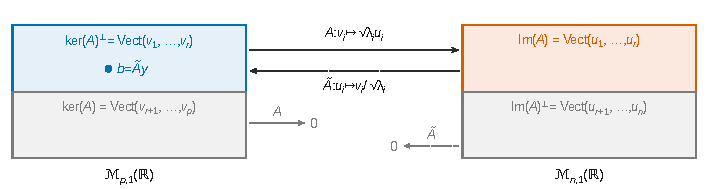
\includegraphics{figures/q42-quatre-sous-espaces.pdf}
\caption*{Figure 4 --- les quatre sous-espaces de la SVD : A envoie ker(A) sur 0
et ker(A)\^{}⊥ bijectivement sur Im(A), Ã fait l'inverse et annule
Im(A)\^{}⊥, donc b = Ãy est dans ker(A)\^{}⊥}
\end{figure}

\hypertarget{question-43}{%
\subsection{Question 43}\label{question-43}}

On écrit \(x_0=b+(x_0-b)\), avec \(b\in(\ker A)^\perp\) (Q42) et \(x_0-b\in\ker A\) (Q41). Par Pythagore,
\equationajustee{\begin{aligned}
\|x_0\|_2^2&=\|b\|_2^2+\|x_0-b\|_2^2\\
&\geqslant\|b\|_2^2,
\end{aligned}}
avec égalité si et seulement si \(x_0-b=0\).
\equationajustee{\boxed{\|x_0\|_2\geqslant\|b\|_2,\ \text{avec \text{égalité} si et seulement si } x_0=b.}}

\hypertarget{partie-e-la-muxe9thode-du-gradient}{%
\section{Partie E --- La méthode du gradient}\label{partie-e-la-muxe9thode-du-gradient}}

Dans cette partie, \(\lambda_1\leqslant\dots\leqslant\lambda_p\) (ordre croissant), tous strictement positifs, et \(S=A^TA\).

\hypertarget{question-44}{%
\subsection{Question 44}\label{question-44}}

\(0\) n'est pas valeur propre de \(S\), donc \(S\) est inversible. Par conséquent \(\ker S=\{0\}\), et \(\ker A=\ker S\) (Q28).
\equationajustee{\boxed{A^TA\text{ inversible et }\ker A=\{0\}.}}

\hypertarget{question-45}{%
\subsection{Question 45}\label{question-45}}

Notons \(\Phi(x,z)=\langle Sx,z\rangle=x^TSz\). \(\Phi\) est bilinéaire.

Elle est symétrique : \(x^TSz\) est un réel, égal à sa transposée \(z^TS^Tx=z^TSx\).

Elle est positive : \(\Phi(x,x)=\|Ax\|_2^2\geqslant0\). Enfin, si \(\Phi(x,x)=0\), alors \(Ax=0\), donc \(x=0\) (Q44). \textbf{\(\Phi\) est un produit scalaire sur \(\mathcal M_{p,1}(\mathbb R)\).}

\hypertarget{question-46}{%
\subsection{Question 46}\label{question-46}}

On a \(\frac14(\alpha+\beta)^2-\alpha\beta=\frac14(\alpha-\beta)^2\geqslant0\), d'où \(\boxed{\alpha\beta\leqslant\frac14(\alpha+\beta)^2.}\)

Comme \(Se_i=\lambda_ie_i\) et \(S^{-1}e_i=\frac1{\lambda_i}e_i\), et la base \((e_i)\) étant orthonormée,
\equationajustee{\begin{aligned}
\langle Sv,v\rangle&=\sum_{i=1}^p\lambda_iv_i^2,\\
\langle S^{-1}v,v\rangle&=\sum_{i=1}^p\frac{v_i^2}{\lambda_i}.
\end{aligned}}
Posons
\equationajustee{\begin{aligned}
\alpha&=\frac1{\lambda_1}\sum_{i=1}^p\lambda_iv_i^2,\\
\beta&=\lambda_p\sum_{i=1}^p\frac{v_i^2}{\lambda_i}.
\end{aligned}}
Alors
\equationajustee{\begin{aligned}
\alpha\beta&=\frac{\lambda_p}{\lambda_1}\langle Sv,v\rangle\langle S^{-1}v,v\rangle,\\
\alpha+\beta&=\sum_{i=1}^p\left(\frac{\lambda_i}{\lambda_1}+\frac{\lambda_p}{\lambda_i}\right)v_i^2.
\end{aligned}}
En multipliant l'inégalité par \(\frac{\lambda_1}{\lambda_p}>0\) :
\equationajustee{\boxed{\langle A^TAv,v\rangle\langle(A^TA)^{-1}v,v\rangle\leqslant\frac14\frac{\lambda_1}{\lambda_p}\left(\sum_{i=1}^p\left(\frac{\lambda_i}{\lambda_1}+\frac{\lambda_p}{\lambda_i}\right)v_i^2\right)^2.}}

\hypertarget{question-47}{%
\subsection{Question 47}\label{question-47}}

\(\psi\) est dérivable sur \([\lambda_1,\lambda_p]\subset\mathbb R_+^*\) et
\equationajustee{\psi'(t)=\frac{t^2-\lambda_1\lambda_p}{\lambda_1t^2}.}
Ainsi \(\psi\) décroît sur \([\lambda_1,\sqrt{\lambda_1\lambda_p}]\) puis croît sur \([\sqrt{\lambda_1\lambda_p},\lambda_p]\). Son maximum est donc atteint en une borne. Or
\equationajustee{\psi(\lambda_1)=1+\frac{\lambda_p}{\lambda_1}=\psi(\lambda_p).}
\equationajustee{\boxed{\max_{[\lambda_1,\lambda_p]}\psi=1+\frac{\lambda_p}{\lambda_1}.}}

\hypertarget{question-48}{%
\subsection{Question 48}\label{question-48}}

Pour tout \(i\), \(\lambda_i\in[\lambda_1,\lambda_p]\), donc
\equationajustee{\frac{\lambda_i}{\lambda_1}+\frac{\lambda_p}{\lambda_i}=\psi(\lambda_i)\leqslant1+c(A).}
Comme \(v_i^2\geqslant0\) et \(\sum v_i^2=\|v\|_2^2\) (base orthonormée), la somme de Q46 est majorée par \((1+c(A))\|v\|_2^2\).

Les deux membres étant positifs, on élève au carré. Avec \(\frac{\lambda_1}{\lambda_p}=\frac1{c(A)}\), on obtient
\equationajustee{\boxed{\langle A^TAv,v\rangle\langle(A^TA)^{-1}v,v\rangle\leqslant\frac{(c(A)+1)^2}{4c(A)}\|v\|_2^4.}}

\hypertarget{question-49}{%
\subsection{Question 49}\label{question-49}}

On a \(S\ell=A^Ty\). Par bilinéarité et symétrie de \(\Phi\),
\equationajustee{\begin{aligned}
\langle S(x-\ell),x-\ell\rangle&=\langle Sx,x\rangle-2\langle Sx,\ell\rangle+\langle S\ell,\ell\rangle\\
&=\langle Sx,x\rangle-2\langle x,A^Ty\rangle+\langle S\ell,\ell\rangle\\
&=f(x)+\langle S\ell,\ell\rangle,
\end{aligned}}
car \(\langle Sx,\allowbreak \ell\rangle=\langle x,\allowbreak S\ell\rangle=\langle x,\allowbreak A^Ty\rangle\). De plus
\equationajustee{f(\ell)=\langle S\ell,\ell\rangle-2\langle\ell,S\ell\rangle=-\langle S\ell,\ell\rangle.}
\equationajustee{\boxed{f(x)-f(\ell)=\langle A^TA(x-\ell),x-\ell\rangle.}}

\hypertarget{question-50}{%
\subsection{Question 50}\label{question-50}}

Posons \(w_k=x_k-\ell\). Comme \(A^Ty=S\ell\), on a \(d_k=Sw_k\), soit \(w_k=S^{-1}d_k\). De plus \(x_{k+1}-\ell=w_k-t_kd_k\). Par Q49,
\equationajustee{f(x_{k+1})-f(\ell)=\Phi(w_k,w_k)-2t_k\Phi(w_k,d_k)+t_k^2\Phi(d_k,d_k).}
Or
\equationajustee{\begin{aligned}
\Phi(w_k,d_k)&=\langle Sw_k,d_k\rangle=\|d_k\|_2^2,\\
\Phi(d_k,d_k)&=\langle Sd_k,d_k\rangle>0\quad(d_k\neq0,\ \text{Q45}).
\end{aligned}}
Donc, avec \(t_k=\frac{\|d_k\|_2^2}{\langle Sd_k,d_k\rangle}\),
\equationajustee{f(x_{k+1})-f(\ell)=\Phi(w_k,w_k)-\frac{\|d_k\|_2^4}{\langle Sd_k,d_k\rangle}.}
Enfin \(\Phi(w_k,\allowbreak w_k)=\langle Sw_k,\allowbreak w_k\rangle=\langle d_k,\allowbreak S^{-1}d_k\rangle=f(x_k)-f(\ell)\). Cette quantité est strictement positive, car \(w_k\neq0\) puisque \(d_k\neq0\). En factorisant :
\equationajustee{\boxed{f(x_{k+1})-f(\ell)=\big(f(x_k)-f(\ell)\big)\left(1-\frac{\|d_k\|_2^4}{\langle A^TAd_k,d_k\rangle\langle(A^TA)^{-1}d_k,d_k\rangle}\right).}}

\begin{figure}[H]
\centering
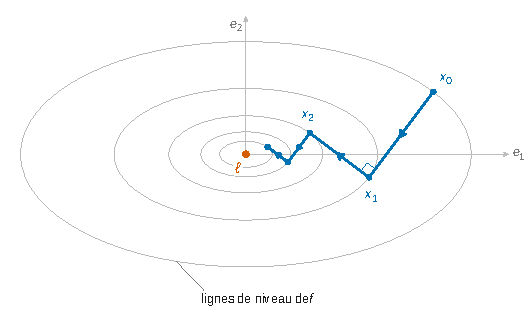
\includegraphics{figures/q50-gradient-zigzag.pdf}
\caption*{Figure 5 --- gradient à pas optimal pour AᵀA = Diag(1, 4) : lignes de
niveau de f elliptiques centrées en ℓ, pas consécutifs orthogonaux,
trajectoire en zigzag vers ℓ}
\end{figure}

\hypertarget{question-51}{%
\subsection{Question 51}\label{question-51}}

\emph{À gauche.} Écrivons \(x_k-\ell=\sum\gamma_ie_i\). Alors
\equationajustee{\begin{aligned}
f(x_k)-f(\ell)&=\sum\lambda_i\gamma_i^2\\
&\geqslant\lambda_1\sum\gamma_i^2\\
&=\lambda_1\|x_k-\ell\|_2^2.
\end{aligned}}

\emph{À droite.} Par Q48 appliquée à \(v=d_k\), les deux membres étant strictement positifs,
\equationajustee{\frac{\|d_k\|_2^4}{\langle Sd_k,d_k\rangle\langle S^{-1}d_k,d_k\rangle}\geqslant\frac{4c(A)}{(c(A)+1)^2},}
donc
\equationajustee{\begin{aligned}
1-\frac{\|d_k\|_2^4}{\langle Sd_k,d_k\rangle\langle S^{-1}d_k,d_k\rangle}&\leqslant1-\frac{4c(A)}{(c(A)+1)^2}\\
&=\left(\frac{c(A)-1}{c(A)+1}\right)^2.
\end{aligned}}
Notons \(q=\left(\frac{c(A)-1}{c(A)+1}\right)^2\). Comme \(f(x_k)-f(\ell)\geqslant0\), Q50 donne
\equationajustee{f(x_{k+1})-f(\ell)\leqslant q\,(f(x_k)-f(\ell)).}
Une récurrence immédiate donne \(f(x_k)-f(\ell)\leqslant q^k(f(x_0)-f(\ell))\).
\equationajustee{\boxed{\lambda_1\|x_k-\ell\|_2^2\leqslant f(x_k)-f(\ell)\leqslant\big(f(x_0)-f(\ell)\big)\left(\frac{c(A)-1}{c(A)+1}\right)^{2k}.}}

\hypertarget{question-52}{%
\subsection{Question 52}\label{question-52}}

\(c(A)=\frac{\lambda_p}{\lambda_1}\geqslant1\), donc \(0\leqslant\frac{c(A)-1}{c(A)+1}<1\) et \(q^k\to0\). Par Q51,
\equationajustee{0\leqslant\|x_k-\ell\|_2^2\leqslant\frac{f(x_0)-f(\ell)}{\lambda_1}q^k\xrightarrow[k\to+\infty]{}0.}
Par encadrement, \(\|x_k-\ell\|_2\to0\), et par le critère admis en fin de partie B, \(\boxed{\lim_{k\to+\infty}x_k=\ell.}\)

Pour tout \(x\), \(\|Ax-y\|_2^2=f(x)+\langle y,y\rangle\). Par Q49, \(f(x)-f(\ell)=\|A(x-\ell)\|_2^2\geqslant0\). Donc \(\|A\ell-y\|_2\leqslant\|Ax-y\|_2\) pour tout \(x\) :
\equationajustee{\boxed{\|A\ell-y\|_2=\min_{x\in\mathcal M_{p,1}(\mathbb R)}\|Ax-y\|_2.}}
(On peut aussi invoquer Q32, puisque \(A^TA\ell=A^Ty\).)

\end{document}
